\documentclass{beamer}
\usetheme{Singapore}
\usepackage{changepage}

%\usepackage{pstricks,pst-node,pst-tree}
\usepackage{amssymb,latexsym,dirtree}
\usepackage{tikz}
\usepackage{graphicx}
\usepackage{fancyvrb}
\usepackage{hyperref}
\usepackage{fancybox}
\usepackage[listings]{tcolorbox}

\definecolor{codegreen}{rgb}{0,0.6,0}
\definecolor{codegray}{rgb}{0.5,0.5,0.5}
\definecolor{codepurple}{rgb}{0.58,0,0.82}
\definecolor{backcolour}{rgb}{0.95,0.95,0.92}

\lstdefinestyle{mystyle}{
    language=Python,
    backgroundcolor=\color{backcolour},   
    commentstyle=\color{codegreen},
    keywordstyle=\color{magenta},
    numberstyle=\tiny\color{codegray},
    stringstyle=\color{codepurple},
    basicstyle=\ttfamily\normalsize,
    breakatwhitespace=false,         
    breaklines=true,                 
    captionpos=b,                    
    keepspaces=true,                 
    numbers=left,                    
    numbersep=5pt,                  
    showspaces=false,                
    showstringspaces=false,
    showtabs=false,                  
    tabsize=2,
    escapechar=|,
    frame=single
}

\lstset{style=mystyle}


\newcommand{\lst}[1]{\lstinline{#1}}

\newcommand{\lsting}[1]{\begin{lstlisting}[basicstyle=#1]}
\newcommand{\lstend}{\end{lstlisting}}

\newcommand{\bi}{\begin{itemize}}
\newcommand{\li}{\item}
\newcommand{\ei}{\end{itemize}}
\newcommand{\Show}[1]{
\begin{center}
\shadowbox{\begin{minipage}{0.8\textwidth}
          #1
          \end{minipage}}
\end{center}
}
\newcommand{\arrow}{\ensuremath{\rightarrow}}

\newcommand{\uparr}{\ensuremath{\uparrow}}


\newcommand{\fig}[2]{\centerline{\includegraphics[width=#1\textwidth]{#2}}}

\newcommand{\bfr}[1]{\begin{frame}[fragile]\frametitle{{ #1 }}}
\newcommand{\efr}{\end{frame}}

\newcommand{\cola}{\begin{columns}\begin{column}{0.5\textwidth}}
\newcommand{\colb}{\end{column}\begin{column}{0.5\textwidth}}
\newcommand{\colc}{\end{column}\end{columns}}


\title{\url{https://intro2r.com/} Chapter 2}
\author{CSCI 297b, Spring 2023}

\begin{document}

\begin{frame}
\maketitle
\end{frame}

\bfr{R basics}
\bi
\li R is case sensitive.  \lst{anova} is not the same as \lst{Anova}
\li Anything following \lst{#} is a comment and is ignored by R
\li Comments should be used liberally
\li Commands are separated by a newline or a semicolon \lst{;}
\li A continuation prompt, \lst{+}, means the previous line is not finished
\li If execution hangs and does not stop, try the escape key or the stop button
\ei
\end{frame}

\bfr{Some builtin R functions}
\begin{lstlisting}[basicstyle=\small]
log(1)              # logarithm to base e
## [1] 0
log10(1)            # logarithm to base 10
## [1] 0
exp(1)              # natural antilog
## [1] 2.718282
sqrt(4)             # square root
## [1] 2
4^2                   # 4 to the power of 2
## [1] 16
pi                    # not a function but useful
## [1] 3.141593
\end{lstlisting}
\end{frame}

\bfr{Objects and assignment}
\begin{lstlisting}
> my_obj <- 1729
> my_obj2 <- "R is cool"
> my_obj
[1] 1729
> my_obj3 <- my_obj / 2
> my_obj3
[1] 864.5
> my_obj4 <- my_obj + my_obj3
> my_obj4
[1] 2593.5
> my_obj5 <- my_obj + my_obj2
Error in my_obj + my_obj2 : non-numeric argument to binary operator
> 
\end{lstlisting}

\end{frame}

\bfr{The Environment Tab}
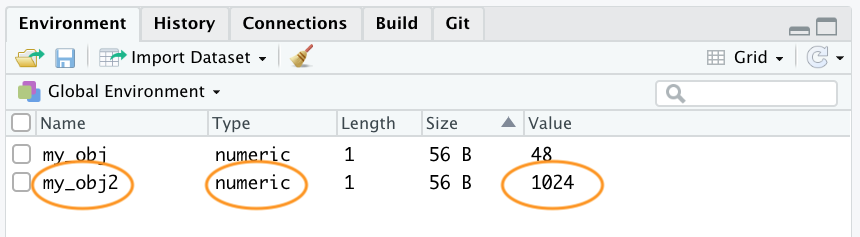
\includegraphics[width=\textwidth]{rs_env}
\end{frame}

\bfr{Naming Objects}

\begin{quotation}
There are two hard problems in computer science: 
cache invalidation, naming things, and off-by-1 errors.

\hfill --- Leon Bambrick
\end{quotation}
\pause

Two often conflicting goals:
\bi
\li Short
\li Meaningful
\ei

\end{frame}

\bfr{Name conventions}

\begin{lstlisting}[basicstyle=\small]
output_summary <- "my analysis"     # snake case
output.summary <- "my analysis"     # dot case
outputSummary <- "my analysis"      # camel case
OutputSummary <- "my analysis"      # Pascal case
output-summary <- "my analysis"     # kebab case
\end{lstlisting}
\bi
\li Snake case used by textbook
\li Google style recommends Pascal for function names
\li Kebab case is illegal in R
\li Dots illegal in many other languages
\li Camel case is my favorite
\ei

\end{frame}

\bfr{Don't use existing names}

\begin{lstlisting}[basicstyle=\small]
data <- read.table("mydatafile", header = TRUE) 
#data is a function!
\end{lstlisting}

\end{frame}
\bfr{The \lst{c()} function}

\lsting{\scriptsize}
my_vec <- c(2,3,1,6,4,3,3,7)
mean(my_vec)    # returns the mean of my_vec
## [1] 3.625
var(my_vec)     # returns the variance of my_vec
## [1] 3.982143
sd(my_vec)      # returns the standard deviation of my_vec
## [1] 1.995531
length(my_vec)  # returns the number of elements in my_vec
## [1] 8
\end{lstlisting}
\end{frame}


\bfr{Sequences}

\lsting{\scriptsize}
my_seq <- 1:10     # create regular sequence
my_seq
##  [1]  1  2  3  4  5  6  7  8  9 10
my_seq2 <- 10:1    # in decending order
my_seq2
##  [1] 10  9  8  7  6  5  4  3  2  1
my_seq2 <- seq(from = 1, to = 5, by = 0.5)
my_seq2
## [1] 1.0 1.5 2.0 2.5 3.0 3.5 4.0 4.5 5.0
my_seq3 <- rep(2, times = 10)   # repeats 2, 10 times
my_seq3
##  [1] 2 2 2 2 2 2 2 2 2 2
my_seq4 <- rep("abc", times = 3)    # repeats 'abc' 3 times 
my_seq4
## [1] "abc" "abc" "abc"
\end{lstlisting}
\end{frame}



\bfr{Sequences}

\lsting{\scriptsize}
my_seq5 <- rep(1:5, times = 3)  # repeats the series 1 to 
                                # 5, 3 times
my_seq5
##  [1] 1 2 3 4 5 1 2 3 4 5 1 2 3 4 5
my_seq6 <- rep(1:5, each = 3)   # repeats each element of 
                                # the series 3 times
my_seq6
##  [1] 1 1 1 2 2 2 3 3 3 4 4 4 5 5 5
my_seq7 <- rep(c(3, 1, 10, 7), each = 3) # repeats each 
                                         # element of the 
                                         # series 3 times
my_seq7
##  [1]  3  3  3  1  1  1 10 10 10  7  7  7

## Alternative approach:
in_vec <- c(3, 1, 10, 7)
my_seq7 <- rep(in_vec, each = 3)   
my_seq7
##  [1]  3  3  3  1  1  1 10 10 10  7  7  7
\end{lstlisting}
\end{frame}


\bfr{Positional indexing}

\lsting{\scriptsize}
my_vec        # remind ourselves what my_vec looks like
## [1] 2 3 1 6 4 3 3 7
my_vec[3]     # extract the 3rd value
## [1] 1

# if you want to store this value in another object
val_3 <- my_vec[3]
val_3
## [1] 1
my_vec[c(1, 5, 6, 8)]
## [1] 2 4 3 7
my_vec[3:8]
## [1] 1 6 4 3 3 7
\end{lstlisting}
\end{frame}


\bfr{Logical indexing}

\lsting{\scriptsize}
my_vec        # remind ourselves what my_vec looks like
## [1] 2 3 1 6 4 3 3 7
my_vec[my_vec > 4]
## [1] 6 7
my_vec > 4
## [1] FALSE FALSE FALSE  TRUE FALSE FALSE FALSE  TRUE
my_vec[c(FALSE, FALSE, FALSE, TRUE, FALSE, FALSE, FALSE, TRUE)]
## [1] 6 7
\end{lstlisting}
\end{frame}

\bfr{Logical indexing}

\lsting{\scriptsize}
my_vec        # remind ourselves what my_vec looks like
## [1] 2 3 1 6 4 3 3 7
my_vec[my_vec >= 4]        # values greater or equal to 4
## [1] 6 4 7
my_vec[my_vec < 4]         # values less than 4
## [1] 2 3 1 3 3
my_vec[my_vec <= 4]        # values less than or equal to 4
## [1] 2 3 1 4 3 3
my_vec[my_vec == 4]        # values equal to 4
## [1] 4
my_vec[my_vec != 4]        # values not equal to 4
## [1] 2 3 1 6 3 3 7
\end{lstlisting}
\end{frame}

\bfr{Boolean expressions}

\begin{Verbatim}[frame=single]
my_vec        # remind ourselves what my_vec looks like
## [1] 2 3 1 6 4 3 3 7
val26 <- my_vec[my_vec < 6 & my_vec > 2]
val26
## [1] 3 4 3 3
val63 <- my_vec[my_vec > 6 | my_vec < 3]
val63
## [1] 2 1 7
\end{Verbatim}
\end{frame}


\bfr{Replacing elements}

\lsting{\scriptsize}
my_vec        # remind ourselves what my_vec looks like
## [1] 2 3 1 6 4 3 3 7

## replace the 4th element with 500
my_vec[4] <- 500
my_vec
## [1]   2   3   1 500   4   3   3   7

# replace the 6th and 7th element with 100
my_vec[c(6, 7)] <- 100
my_vec
## [1]   2   3   1 500   4 100 100   7

# replace element that are less than or equal to 4 with 1000
my_vec[my_vec <= 4] <- 1000
my_vec
## [1] 1000 1000 1000  500 1000  100  100    7
\end{lstlisting}
\end{frame}

\bfr{Sorting elements}

\lsting{\scriptsize}
my_vec
## [1] 1000 1000 1000  500 1000  100  100    7

vec_sort <- sort(my_vec)
vec_sort
## [1]    7  100  100  500 1000 1000 1000 1000

vec_sort2 <- sort(my_vec, decreasing = TRUE)
vec_sort2
## [1] 1000 1000 1000 1000  500  100  100    7

vec_sort3 <- rev(sort(my_vec))
vec_sort3
## [1] 1000 1000 1000 1000  500  100  100    7
\end{lstlisting}
\end{frame}

\bfr{Ordering elements}

\lsting{\scriptsize}
height <- c(180, 155, 160, 167, 181)
height
## [1] 180 155 160 167 181

p.names <- c("Joanna", "Charlotte", "Helen", "Karen", "Amy")
p.names
## [1] "Joanna"    "Charlotte" "Helen"     "Karen"     "Amy"

height_ord <- order(height)
height_ord
## [1] 2 3 4 1 5

 height[height_ord]
## [1] 155 160 167 180 181

names_ord <- p.names[height_ord]
names_ord
## [1] "Charlotte" "Helen"     "Karen"     "Joanna"    "Amy"
\end{lstlisting}
\end{frame}


\bfr{Vectorization}

\lsting{\scriptsize}
# create a vector
my_vec2 <- c(3, 5, 7, 1, 9, 20)

# multiply each element by 5
my_vec2 * 5
## [1]  15  25  35   5  45 100

# create a second vector
my_vec3 <- c(17, 15, 13, 19, 11, 0)

# add both vectors
my_vec2 + my_vec3
## [1] 20 20 20 20 20 20

# multiply both vectors
my_vec2 * my_vec3
## [1] 51 75 91 19 99  0
\end{lstlisting}
\end{frame}

\bfr{Vectorization recycling}

\lsting{\scriptsize}
my_vec2 <- c(3, 5, 7, 1, 9, 20)
my_vec4 <- c(1, 2)

# add both vectors - quiet recycling!
my_vec2 + my_vec4
## [1]  4  7  8  3 10 22
\end{lstlisting}
\end{frame}


\bfr{Missing data}

\lsting{\scriptsize}
temp  <- c(7.2, NA, 7.1, 6.9, 6.5, 5.8, 5.8, 5.5, NA, 5.5)
temp
##  [1] 7.2  NA 7.1 6.9 6.5 5.8 5.8 5.5  NA 5.5

mean_temp <- mean(temp)
mean_temp
## [1] NA

mean_temp <- mean(temp, na.rm = TRUE)
mean_temp
## [1] 6.2875
\end{lstlisting}

\bi
\li Some functions may deal with NAs differently.
\li Always consult the documentation.
\ei
\end{frame}


\bfr{R help}

\lsting{\scriptsize}
## show the help page:
help("mean")
?mean

## search all help pages:
help.search("mean")
??mean
\end{lstlisting}

\bi
\li Also use the Help tab in RStudio
\li Usually the most helpful part of a help page is the examples.
\ei

\end{frame}


\bfr{R help}

\lsting{\tiny}
apropos("mean")
##  [1] ".colMeans"     ".rowMeans"     "colMeans"      "kmeans"       
##  [5] "mean"          "mean_temp"     "mean.Date"     "mean.default" 
##  [9] "mean.difftime" "mean.POSIXct"  "mean.POSIXlt"  "rowMeans"     
## [13] "vec_mean"      "weighted.mean"
\end{lstlisting}

\bi
\li Find all functions with "mean" in their name.
\ei



\lsting{\scriptsize}
RSiteSearch("regression")
\end{lstlisting}

\bi
\li Search  for keywords and phrases in function help pages and vignettes for all CRAN packages, and in CRAN task views.
\ei

\end{frame}

\bfr{General R resources}

\bi
\li
\url{https://cran.r-project.org/other-docs.html}

R-Project: User contributed documentation


\li
\url{https://journal.r-project.org/}

The R Journal: Journal of the R project for statistical computing


\li
\url{http://swirlstats.com/}

Swirl: An R package that teaches you R from within R


\li
\url{https://www.rstudio.com/resources/cheatsheets/}

RStudio’s printable cheatsheets

\li
\url{http://rseek.org/}

Rseek A custom Google search for R-related sites

\ei

\end{frame}

\bfr{Getting help}

\bi
\li
\url{https://www.google.com/}

Google it!: Try Googling any error messages you get. It’s not cheating and everyone does it! You’ll be surprised how many other people have probably had the same problem and solved it.

\li
\url{http://stackoverflow.com/questions/tagged/r}

Stack Overflow: There are many thousands of questions relevant to R on Stack Overflow. Here are the most popular ones, ranked by vote. Make sure you search for similar questions before asking your own, and make sure you include a reproducible example to get the most useful advice. A reproducible example is a minimal example that lets others who are trying to help you to see the error themselves.
\ei

\end{frame}


\bfr{Saving stuff}
\bi
\li Normally the only thing you need to save is your R script.
\li Put everything you do in the script.
\li Save it, and the next time you start just source it.
\ei

\end{frame}


\bfr{Global options}
\cola
\begin{itemize}
\item \fbox{\sf Tools}\arrow\fbox{\sf Global Options ...}

\item
Turn off \verb|.RData| save and restore
\item
This prevents new R sessions from being influenced
by previous R sessions.
\end{itemize}

\colb
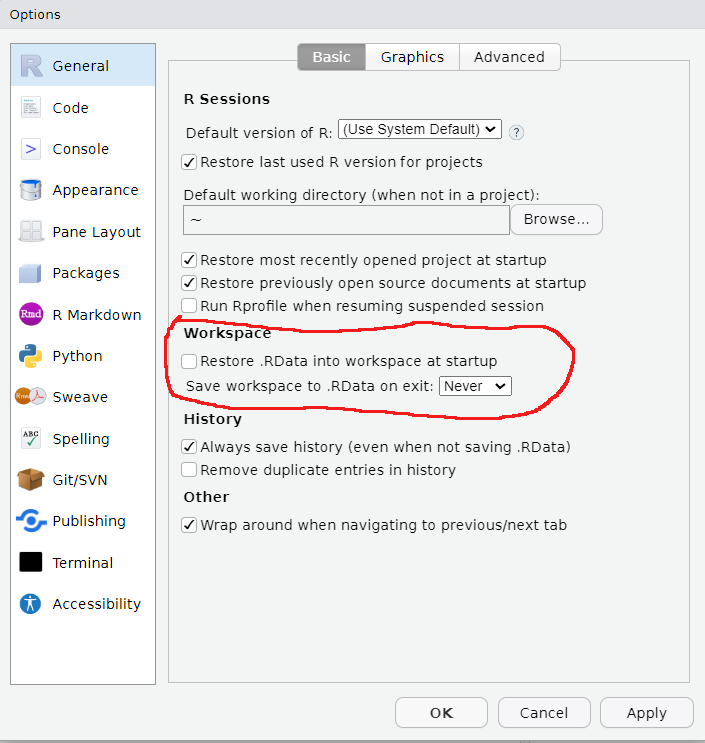
\includegraphics[width=\textwidth]{globaloptions}
\colc
\end{frame}

\bfr{Saving objects}
\bi
\li Occasionally you want to save an object rather than recompute it.
\li Some objects may take minutes or hours to compute.
\ei
\lsting{\scriptsize}
## save a single object to a file
save(nameOfObject, file = "name_of_file.RData")

## save all the objects in your workspace in a single file
save.image(file = "name_of_file.RData")

## reload whatever you saved
load(file = "name_of_file.RData")
\end{lstlisting}
\end{frame}

\end{document}
